\documentclass[11pt]{article}
\usepackage{amsmath}
\usepackage{fancyhdr}
\usepackage{hyperref}
\usepackage{graphicx}

\usepackage{mathtools}
\usepackage{pst-node}

\newcommand{\compactlist}{\setlength{\itemsep}{0pt} \setlength{\parskip}{0pt} \setlength{\leftskip}{-1em}}
\usepackage[top=0.9in, bottom=0.8in, left=0.9in, right=0.9in]{geometry}

\lhead{MATH 4363/5373}
\rhead{Dec. 4, 2019}
\chead[RE]{Monte Carlo integration}
\cfoot{}
%\rfoot{Code for figure and report is available in the class folder.}
\pagestyle{fancy}
\begin{document}

\textit{This section may be imperfect, but reflects the main idea.}

Though not emphasized here, the techniques that follow are most useful in higher dimensional integrals. We can integrate \(f(x) = x^2\) using the Fundamental Theorem of Calculus,
\[\int_0^2 x^2\,dx = \left.\left(\dfrac{x^3}{3}\right)\right|_0^2 = \dfrac{2^3}{3} - \dfrac{0^3}{3} = \dfrac{8}{3}\]
From the Mean Value Theorem for Integrals we have that \[\hat{f} = \dfrac{1}{2-0}\int_0^2 x^2\,dx = \dfrac{1}{2}\cdot \dfrac{8}{3} = \dfrac{4}{3}\]
The shaded region on the left panel (Fig~\ref{fig::calc}) shows the area under the curve. The area on the right is the same size, but bounded by a constant function whose value is \(\hat{f}\).

\begin{figure}[h!]\centering
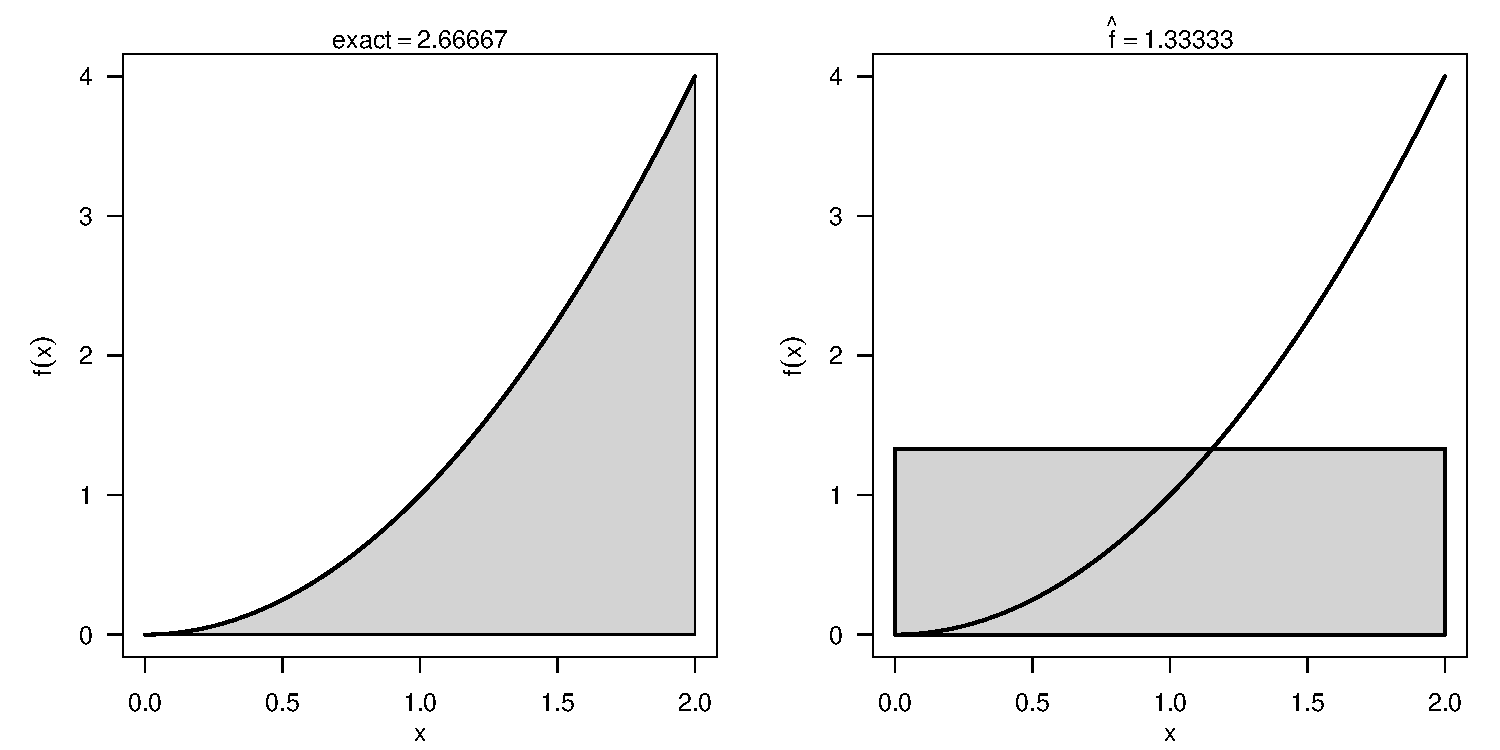
\includegraphics[width=0.9\textwidth]{intro.pdf}
\caption{Left: Traditional calculus interpretation of the area under the curve. Right: Average value of a function defined by equal area.}\label{fig::calc}
\end{figure}

One scheme of Monte Carlo integration uses function values at randomly chosen points to calculate areas which are then averaged. Here \[\int_a^b f(x)\,dx \approx \dfrac{1}{N}\sum_{i=1}^{N} \underbrace{(b-a)f(x_i)}_\text{\(i\)th area} = (b-a)\underbrace{\dfrac{1}{N}\sum_{i=1}^{N} f(x_i)}_\text{average height}\] Fig~\ref{fig::average} (left panel) shows 5 of the 100 random rectangle regions. The shaded area on the right panel corresponds to the region whose height is the average of the random function values. Notice that this height very closely compares with the average value of the function, thus the areas of the regions are similar.
%
\begin{figure}[h!]\centering
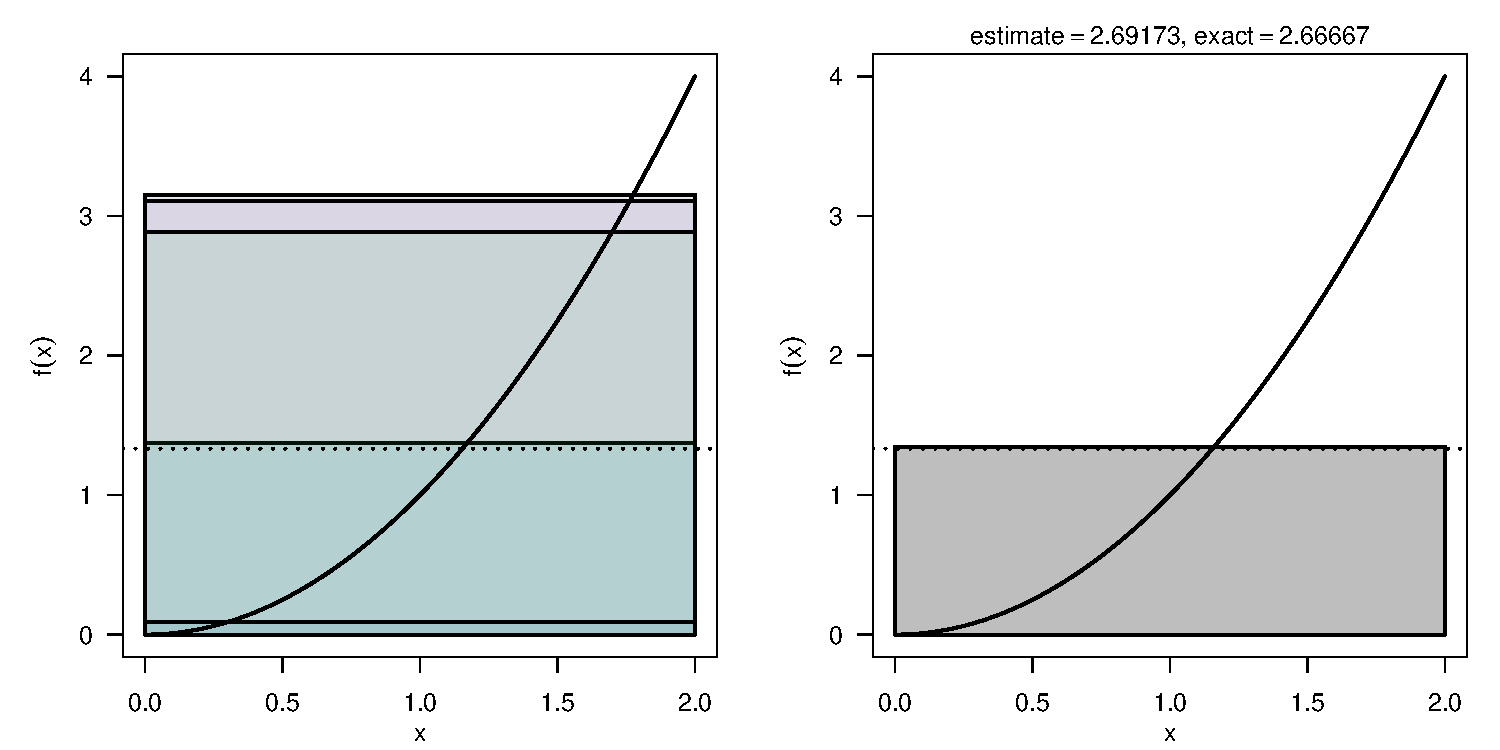
\includegraphics[width=0.9\textwidth]{rectangles.pdf}
\caption{Dashed line indicates \(\hat{f}\) from traditional calculus. Left: 5 sample rectangles (shaded). Right: Average area and function height by random sampling.}\label{fig::average}
\end{figure}

An alternate scheme (Fig~\ref{fig::compare}, left) plots points in the plane and considers the fraction of points that fall below the curve (i.e., `the acceptance region`). This fraction is multiplied by the total area of the region (easier to calculate since the shape is likely square). Though this is easier to program than the notation might suggest, consider the indicator function \[I(i) = \begin{cases}1, \quad y_i < f(x_i)\\0, \quad\text{otherwise}\end{cases}\]~and take~\[\int_a^b f(x)\,dx \approx(f_{max}-f_{min})(b-a)\dfrac{1}{N} \sum_{i=1}^N I(i)\]
%
\begin{figure}[h!]\centering
\begin{minipage}{0.48\textwidth}\centering
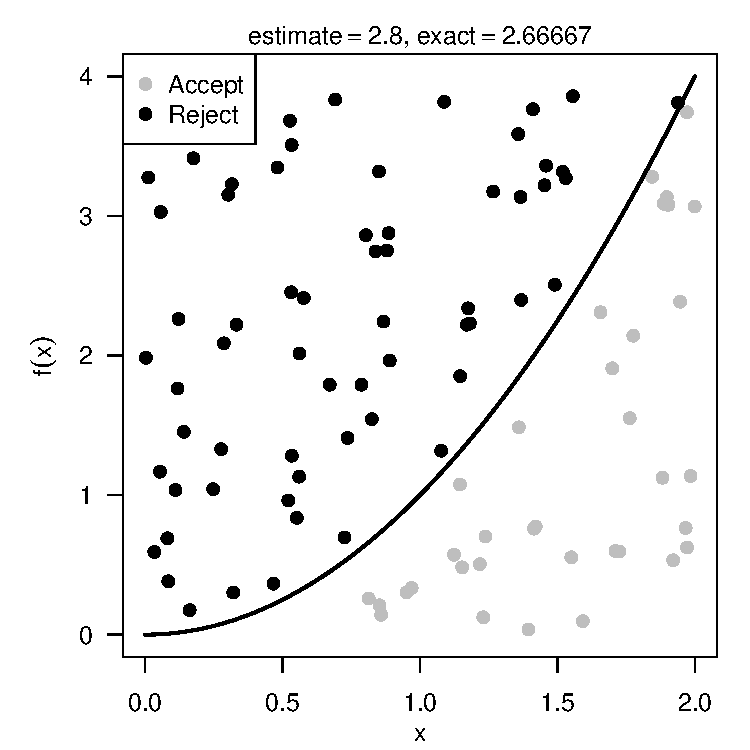
\includegraphics[width=0.9\textwidth]{rejection.pdf}

\end{minipage}
\begin{minipage}{0.48\textwidth}

\centering
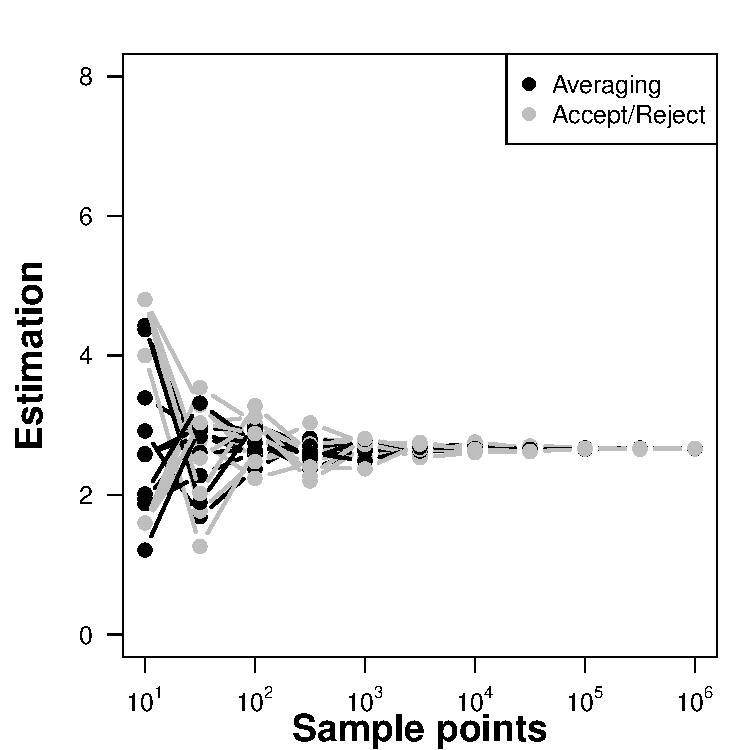
\includegraphics[width=0.9\textwidth]{Ns.pdf}
\end{minipage}
\caption{Left: Accepted points fall below the graph of the function. Right: Comparison of rectangle method and rejection method for ten different trials of each.}\label{fig::compare}
\end{figure}


\end{document}
